\section{Performance evaluation}
\label{sec:evaluation}
% Trung & Le's text
%In this section, we perform experiments to evaluate the performance of MuLeS and compare it with four baselines, namely minRTT, BLEST, ECF, and Peekaboo.

% Kien 's text
In this section, we evaluate the performance of MuLeS in comparison to four baselines (i.e., minRTT, BLEST, ECF, and Peekaboo).


\subsection{Settings}
\label{subsec:experiment}
%We use Mininet-WiFi~\cite{mininetwifi} to emulate a multipath environment, which follows the topology illustrated in~\figref{fig:networkmodel}. The network includes an MPQUIC server connecting to network devices (including Access Point and Base Station) via wired links, three MPQUIC clients via Wi-Fi, and LTE/5G interfaces. The bandwidth of the wired links is set in the range of 30-80Mbps to match current connections, according to Ookla's Speedtest Global Index~\cite{speedtest}. The average latency, latency variability, and data loss rates are based on a study by Microsoft~\cite{microsoft}. We summarize wired link parameters in Table \ref{tab1}. Moreover, we use \textit{wmediumd} with the Log Distance Propagation Loss Model to create wireless links~\cite{10.1145/3568562.3568654}. We run 100 experiments per scenario for each scheduler on an Ubuntu 22.04 (4-core CPU, 8G RAM). We consider download time in different file download scenarios as a metric to evaluate the performance of five schedulers. In all of our experiments, we set the file size to 4MB. We conduct four main experiments to evaluate (i) efficiency of MuLeS in dealing with the selfish scheduling phenomenon, (ii) impacts of packet loss rate, (iii) impacts of RTT variation, and (iv) impacts of network dynamicity level.

%  Kien slighlty modified Sep. 3
We use Mininet-WiFi~\cite{mininetwifi} to emulate a multipath environment following the model in~\figref{fig:networkmodel}. The network includes an MPQUIC server connecting to a simulated Access Point and a Base Station via wired links. Moreover, three MPQUIC clients use their Wi-Fi and LTE interfaces to connect to the wireless networks. The wired links' bandwidth is set in the range of 30-80Mbps to match current connections, according to Ookla's Speedtest Global Index~\cite{speedtest}. The average latency, latency variability, and data loss rates are based on the previous studies~\cite{microsoft,wifi,4g}. We summarize wired link parameters in Table \ref{tab1}. Moreover, we use \textit{wmediumd} with the Log Distance Propagation Loss Model to create wireless links~\cite{10.1145/3568562.3568654}. We run 100 experiments per scenario for each scheduler on an Ubuntu 22.04 (4-core CPU, 8G RAM). We consider download time in different file download scenarios as a metric to evaluate the performance of five schedulers. 
In all of our experiments, we set the file size to 4MB. We conduct four main experiments to evaluate (i) efficiency of MuLeS in dealing with the rush scheduling phenomenon; (ii) impacts of packet loss rate; (iii) impacts of RTT variation; and (iv) impacts of network dynamicity level.

\begin{table}[t]
\begin{center}
\caption{Path parameters.}
\label{tab1}
\begin{tabular}{|c|c|c|}
\hline
% \textbf{}&\multicolumn{2}{c|}{\textbf{Server} (and)} \\
% \cline{2-3} 
\textbf{} & \textbf{Base Station}& \textbf{Access Point} \\
\hline
Bandwidth (Mbps)& 30 (up to 35)& 55 (up to 60)   \\
\hline
RTT (ms)& 20& 30  \\
\hline
\end{tabular}
\end{center}
%\vspace{-0.3cm}
\end{table}


\subsection{Experimental results}
\label{subsec:numerical}
\begin{figure}[ht!]
\centering
\hspace{2em}
\includegraphics[width=0.45
\linewidth]{figs/leg.eps}
   \subfloat[minRTT.\label{fig:selfishrtt} ]{%
      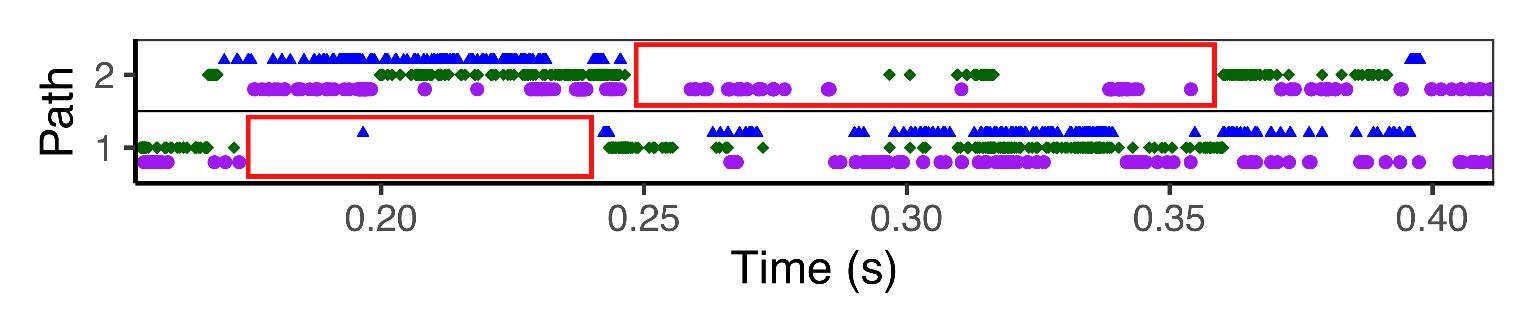
\includegraphics[ width=\linewidth]{figs/RTT.eps}}\\
   \subfloat[MuLeS.\label{fig:selfishmules}]{%
      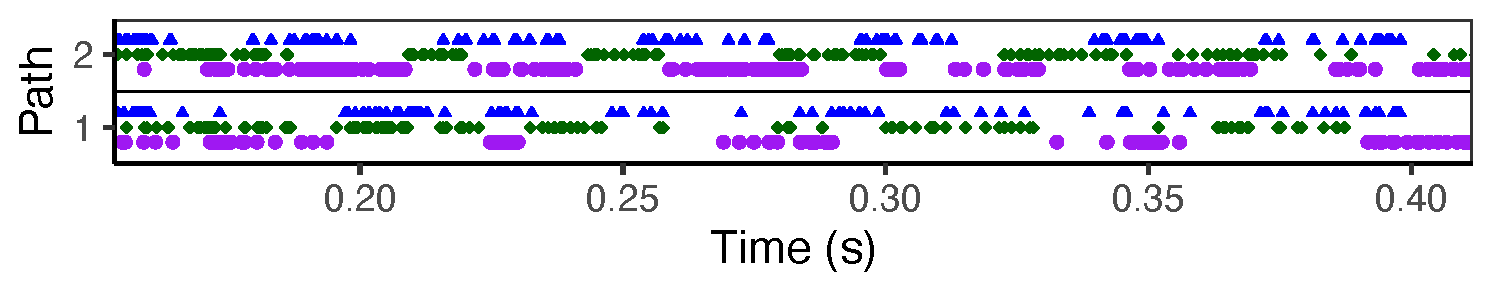
\includegraphics[width=0.98\linewidth]{figs/MuLeS.eps}}\\
\caption{\textbf{Comparison of path utilization between minRTT and MuLeS.} minRTT tends to choose the lower-RTT path, resulting in congestion in this path, while leaving the other path unused (\textcolor{red}{red rectangle areas}). MuLeS, on the other hand, leverages the advantage of both paths for all sessions, thereby eliminating biased usage.}
    \label{fig:Selfish2}
\end{figure}

\begin{figure*}[ht!]
\centering
\hspace{2em}
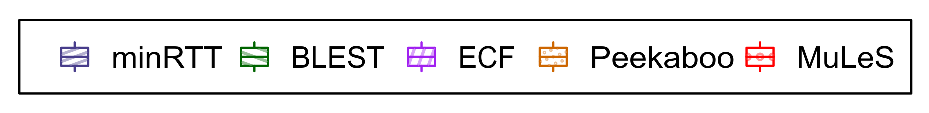
\includegraphics[width=0.4
\textwidth]{figs/loss_leg.eps}\linebreak
   \subfloat[Impacts of loss rate \label{fig:loss_rate}]{%
      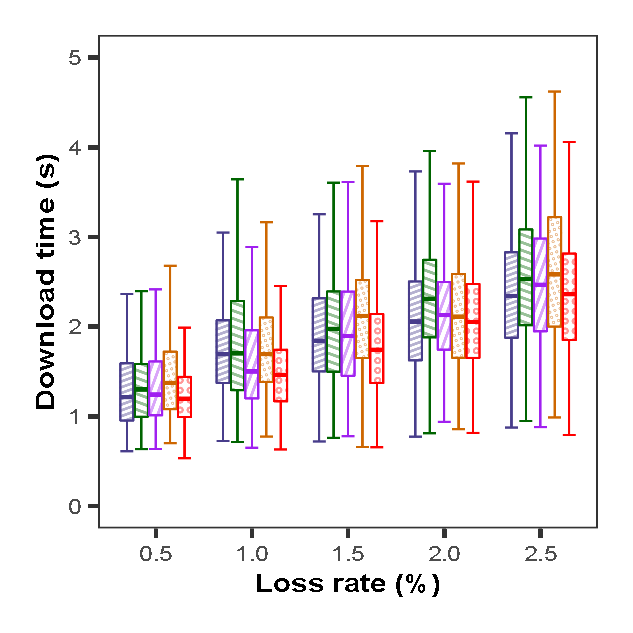
\includegraphics[ width=0.31\textwidth]{figs/loss.eps}}
\hspace{1em}
   \subfloat[Impacts of RTT variation \label{fig:rtt_variation} ]{%
      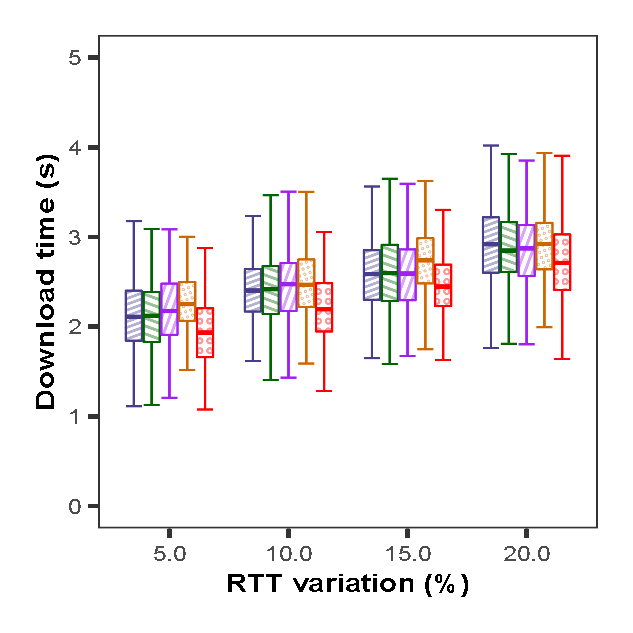
\includegraphics[ width=0.31\textwidth]{figs/vRTT.eps}}
\hspace{1em}
   \subfloat[Impacts of dynamicity level \label{fig:dynamic}]{%
      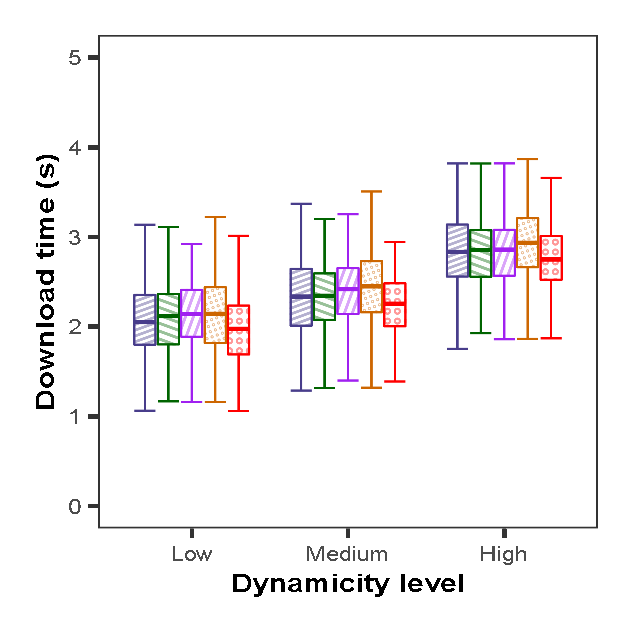
\includegraphics[ width=0.31\textwidth]{figs/dyn.eps}}\\
\caption{Comparison of the MPQUIC schedulers' download when varying loss rate, RTT variations, and dynamicity level.}
    \label{fig:lossrtt}
\end{figure*}


% Kien's text Sep. 03
In this evaluation, we examine the MPQUIC schedulers under different network conditions. Moreover, based on an empirical study, we chose the following hyperparameters for MuLeS: learning rate $\alpha = 0.6$, discount factor $\gamma = 0.6$, $\beta = 9$, and $\varepsilon = 0.4$.

\noindent \textbf{Alleviating the rush scheduling phenomenon:} Since all the comparison benchmarks follow the logic of minRTT, in the following, we choose minRTT as the representative and present the comparison between minRTT and MuLeS against the rush scheduling phenomenon. \figureref{fig:selfishrtt} visualizes the paths selected by minRTT in a certain period.
As shown, due to the rush scheduling phenomenon, in some time slots, the schedulers of all sessions strive for the same path while leaving the other one vacant. To be more specific, from 0.15 to 0.22 seconds, the three sessions chose Path 2 while leaving Path 1 unused. In contrast, during 0.25-0.36 seconds, all sessions focus on Path 1 while leaving Path 2 vacant. On the other hand, MuLeS can consider all sessions' states when making scheduling decisions. Therefore, it can balance the workload imposed on the two paths, thereby alleviating the rush scheduling phenomenon.

% Kien's text 2023 Sep. 03
\noindent \textbf{Impacts of loss rate:} In this evaluation, we fix the RTT variation and vary the packet loss rate between 0\% and 2.5\%. The download time results are shown in~\figref{fig:loss_rate}. We can observe that MuLeS outperforms the other schedulers. Notably, when the expected loss is 1.5\%, MuLeS reduces the download time by 8\% compared to the others. However, when the expected loss is higher (e.g., 2.5\%), the performance gap between MuLeS and minRTT-based becomes less significant. 

%\noindent \textbf{Impacts of RTT variation:}
%In this section, we study the impacts of RTT variation by varying its value from 5.0\% to 20\% with 5\% and plot the download time of the schedulers on~\figref{fig:rtt_variation}.
%As shown, MuLeS reduces the download time significantly compared to the other benchmarks.
%%Next, we investigate the impact of RTT variation while keeping the loss rate fixed. RTT variation ranges from 5.0\% to 20\% with 5\% granularity. Figure \ref{fig:rtt_variation} displays the results, illustrating the clear advantage of MuLeS over the other benchmarks. 
%While minRTT, ECF, BLEST, and Peekaboo suffer from increased download times as RTT variation rises, MuLeS maintains stable performance due to its adaptability. 
%Moreover, MuLeS's design, based on lightweight multi-client learning, allows it to observe and evaluate network state instantaneously. 
%As a result, across all scenarios, MuLeS consistently achieves download times 9-16\% lower than the other schedulers, showcasing its superior adaptability even in cases of high RTT variation (up to 20\%). 

% Kien slightly modified Sep. 03
\noindent \textbf{Impacts of RTT variation:} This evaluation studies the impacts of RTT variation by varying its value from 5.0\% to 20\% with a 5\% increasing step. We plot the download time of the schedulers in~\figref{fig:rtt_variation}. As shown, MuLeS reduces the download time significantly compared to the others. While minRTT, ECF, BLEST, and Peekaboo suffer from increased download times as the RTT variation rises, MuLeS maintains stable performance due to its adaptability. Moreover, MuLeS, with lightweight multi-client learning, allows it to observe and evaluate network state instantaneously. As a result, across all scenarios, MuLeS consistently achieves download times 9-16\% lower than the others.%, showcasing its superior adaptability.
%even in cases of high RTT variation (up to 20\%). 

\begin{table}[t]
\begin{center}
\caption{Dynamicity level.}
\label{tab2}
\begin{tabular}{|c|c|c|c|}
\hline
\textbf{}&\multicolumn{3}{|c|}{\textbf{Dynamicity level}} \\
\cline{2-4} 
\textbf{} & \textbf{\textit{Low}}& \textbf{\textit{Medium}}& \textbf{\textit{High}} \\
\hline
RTT variation (\%)& 5& 10& 20   \\
\hline
Loss rate (\%)& 0.1& 0.5& 0.9  \\
\hline
\end{tabular}
\end{center}
%\vspace{-0.5cm}
\end{table}
\noindent \textbf{Impacts of dynamicity level:}
Lastly, we assess the performance of the schedulers under different dynamicity levels, categorized as Low, Medium, and High, as detailed in Table~\ref{tab2}. The results, depicted in~\figref{fig:dynamic}, indicate that as the dynamic level increases, minRTT, ECF, BLEST, and Peekaboo exhibit weaknesses in adapting to network fluctuations, leading to rapid growth in download times. In contrast, MuLeS demonstrates better adaptability under varying conditions. Compared to Peekaboo, MuLeS improves performance by 7\% to 11\%. Additionally, the cumulative distribution function (CDF) of download time on each client, shown in~\figref{fig:dynamiccdf}, reveals that the performance of MuLeS is better than the other schedulers in different dynamicity levels. This result shows that MuLeS optimizes global download time and ensures optimal local download time per session.

In summary, MuLeS proves its capability to adapt to wireless networks'
dynamicity and capturing the states of all sessions to make appropriate scheduling decisions for all clients simultaneously. MuLeS reduces the download time significantly compared to all other schedulers in all scenarios.

\begin{figure}[ht!]
\hspace*{2.1em}
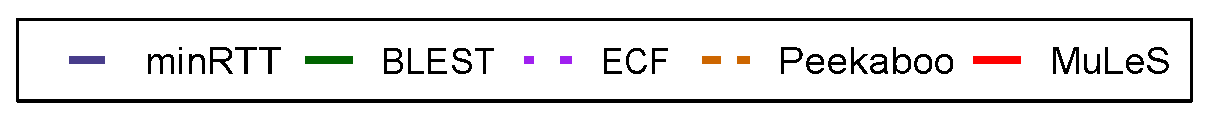
\includegraphics[width=0.44
\textwidth]{figs/dyn_leg.eps}\\
\centering
   \subfloat[Low - Client 1 \label{fig:low_c0}]{%
      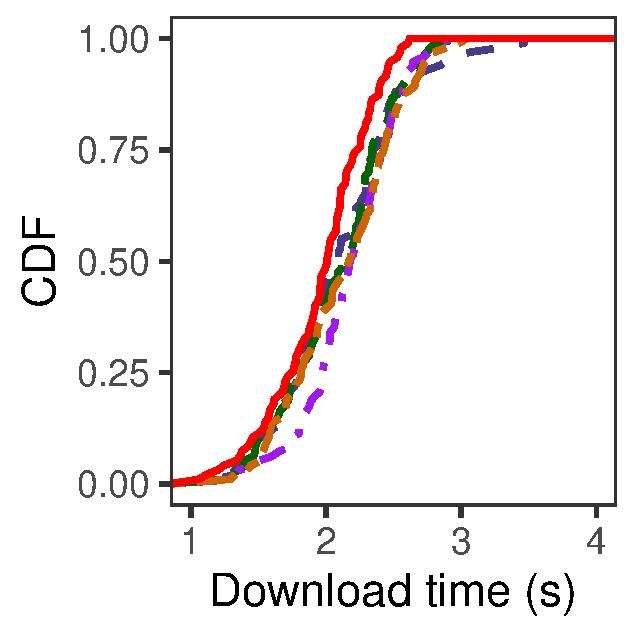
\includegraphics[ height=0.38\linewidth]{figs/low_c0.eps}}
\hspace{0em}
   \subfloat[Low - Client 2 \label{fig:low_c1} ]{%
      \includegraphics[ height=0.38\linewidth]{figs/low_c1.eps}}
\hspace{0em}
   \subfloat[Low - Client 3 \label{fig:low_c2}]{%
      \includegraphics[ height=0.38\linewidth]{figs/low_c2.eps}}\\
   \subfloat[Medium - Client 1 \label{fig:medium_c0}]{%
      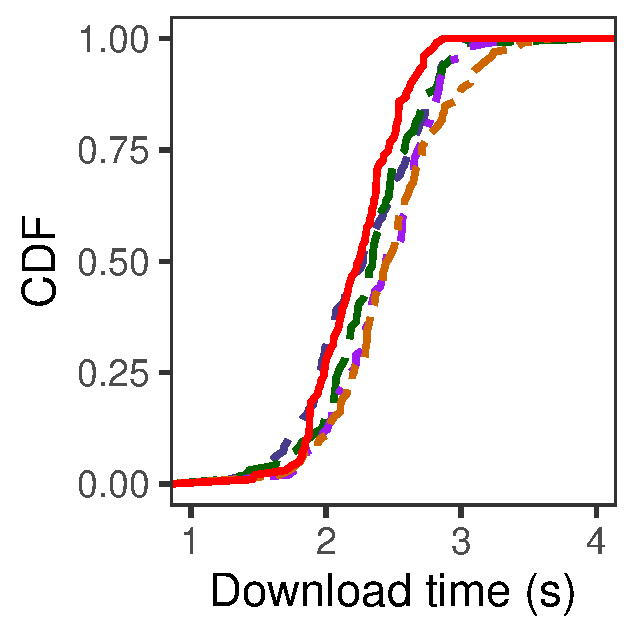
\includegraphics[ height=0.38\linewidth]{figs/medium_c0.eps}}
\hspace{0em}
   \subfloat[Medium - Client 2 \label{fig:medium_c1} ]{%
      \includegraphics[ height=0.38\linewidth]{figs/medium_c1.eps}}
\hspace{0em}
   \subfloat[Medium - Client 3 \label{fig:medium_c2}]{%
      \includegraphics[ height=0.38\linewidth]{figs/medium_c2.eps}}\\
   \subfloat[High - Client 1 \label{fig:high_c0}]{%
      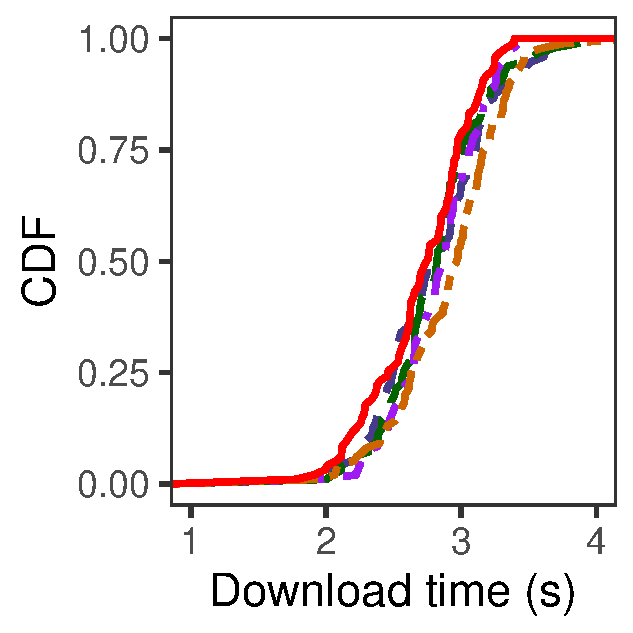
\includegraphics[ height=0.38\linewidth]{figs/high_c0.eps}}
\hspace{0em}
   \subfloat[High - Client 2 \label{fig:high_c1} ]{%
      \includegraphics[ height=0.38\linewidth]{figs/high_c1.eps}}
\hspace{0em}
   \subfloat[High - Client 3 \label{fig:high_c2}]{%
      \includegraphics[ height=0.38\linewidth]{figs/high_c2.eps}}\\
\caption{Download times of each client in different dynamicity levels.}
    \label{fig:dynamiccdf}
\end{figure}
